\documentclass{../tuda-exercise}

% Title information
\version{28. März 2022}
\sheetnumber{7}

\begin{document}

  \maketitle

  \begin{task}[credit=\stars{0}{3}]{Theoriefragen}
    \begin{subtask*}{Grundlegendes}
      \begin{enumerate}
        \item Wie hängen die Begriffe \inlinejava{throws} und \inlinejava{throws} zusammen? Wo
        wird was verwendet?
        \item Ist es sinnvoll, eigene Exceptionklassen zu definieren? Welche Vorteile ergeben
        sich hieraus?
        \item Nennen Sie die Methoden der \inlinejava{Assert}-Klasse, die Sie zum Testen bei
        einem typischen JUnit
        Testcase in der Vorlesung kennengelernt haben, und beschreiben Sie kurz deren Verwendung.
      \end{enumerate}

      \begin{solution}
        \begin{enumerate}
          \item \inlinejava{throws} wird im Methodenkopf verwendet, um zu signalisieren, dass
          eine Methode eine Exception dieser Klasse wirft.
          \\
          \inlinejava{throws} hingegen wird in der Methode verwendet, um eine Exception mit
          \inlinejava{throw new Exception()} zu werfen (dabei kann statt Exception auch eine von
          Exception abgeleitete Klasse stehen). Falls eine \inlinejava{Exception} geworfen wird,
          so wird die momentane Ausführung der Methode unterbrochen. \inlinejava{Exception}
          bieten die Möglichkeit, wenn etwas Ungewöhnliches im Programm geschieht, diese Tatsache
          von der Hauptlogik eines Programms zu trennen. Durch eine \inlinejava{Exception} kann
          dadurch die Ursache des Fehlers vor allem schneller gefunden werden.
          \item Bei eigenen Exception-Klassen können Informationen an den Konstruktor übergeben
          werden, was die Fehlerbehandlung erleichtern kann und zum Beispiel für eine
          detaillierte Ausgabe der Probleme sorgt.

          \br

          Ein weiterer Grund für eigene Exception-Klassen ist, dass der Name damit häufig schon
          die wesentliche Information enthalten kann, z.B. der Name
          \inlinejava{ArrayIndexOutOfBoundsException} sagt zusammen mit dem Call-Stack eigentlich
          schon alles, was man über den Fehler wissen muss.
          \item
          \begin{itemize}
            \item \inlinejava{assertEquals}(erwarteter Wert, tatsächlicher Wert, (ggf. Abweichung)):
            \\
            Die Methode liefert einen Fehler, wenn sich die beiden Werte unterscheiden (bzw. wenn
            sie sich um mehr als die Abweichung unterscheiden)
            \item \inlinejava{assertTrue}(Prädikat/boolescher Wert):
            \\
            Die Methode liefert einen Fehler, wenn false zurückliefert wird

            \clearpage

            \item \inlinejava{assertThrows}(Exceptionname.\textcolor{keywordcolor}{class},
            Executable Lambda-Ausdruck):
            \\
            Die Methode liefert einen Fehler, wenn die Exception nicht geworfen wird

            \br

            Dazu ein paar Hintergrundinformationen zu Executable. Einmal das Interface von
            Executable:

            \lstinputlisting[style=Java]{codes/V1_13_Solution.java}
            \begin{itemize}
              \item Jetzt noch der formale Aufbau, wie man einen Executable Lambda-Ausdruck
              definieren könnte:
              \begin{center}
                \inlinejava{Executable example = () -> \{Operationen;\};}
              \end{center}
            \end{itemize}
          \end{itemize}
        \end{enumerate}

        \begin{note}[title=Information:]
          Mehr Informationen zu \inlinejava{Assertions} finden Sie unter dem folgenden Verweis:

          \begin{center}
            \url{https://junit.org/junit5/docs/5.0.1/api/org/junit/jupiter/api/Assertions.html}
          \end{center}
        \end{note}
      \end{solution}
    \end{subtask*}

    \begin{subtask*}{Wahr oder falsch?}
      Welche der folgenden Aussagen ist wahr?
      \begin{enumerate}
        [label=(\Alph*)]
        \item Auf einen \inlinejava{try}-Block muss immer mindestens ein \inlinejava{catch}-Block
        folgen.
        \item Wenn Sie eine Methode schreiben, die eine Exception auslösen könnte, müssen Sie
        diesen riskanten Code mit einem \inlinejava{try}/\inlinejava{catch}-Block umgeben.
        \item Auf einen \inlinejava{try}-Block können beliebig viele verschiedene
        \inlinejava{catch}-Blöcke folgen.
        \item Eine Methode kann nur eine einzige Art von Exception werfen.
        \item Die Reihenfolge der \inlinejava{catch}-Blöcke ist grundsätzlich gleich gültig.
        \item Laufzeit (Runtime)-Exceptions müssen gefangen oder deklariert werden.
        \item Es darf kein Code zwischen dem \inlinejava{try}-Block und dem
        \inlinejava{catch}-Block geschrieben werden.
        \item Eine Methode wirft eine Exception mit dem Schlüsselwort \inlinejava{throws}.
      \end{enumerate}

      \begin{solution}
        \begin{enumerate}
          [label=(\Alph*)]
          \item Ein \inlinejava{try}-Block kommt nie allein, sondern immer mit einem oder
          manchmal mehreren \inlinejava{catch}-Blöcken, die unmittelbar danach kommen. Die
          einzigen Ausnahmen sind, wenn nach einem \inlinejava{try}-Block ein
          \textcolor{keywordcolor}{finally}-Block\footnote{Das Schlüsselwort wurde nicht in der
          Vorlesung behandelt und es wird abgeraten es zu verwenden} folgt oder es sich um einen
          \textcolor{keywordcolor}{try-with-resources}-Block handelt.
          \item Der riskante Code muss nicht von einem \inlinejava{try}/\inlinejava{catch}-Block
          umgeben werden, weil Exceptions auch weitergerreicht werden können. Eine weitere
          Ausnahme sind Runtime Exception oder die abgeleiteten Klassen, weil sie auch ohne einen
          \inlinejava{try}/\inlinejava{catch}-Block geworfen werden.
          \item Ja, solange zwischen denen kein Code steht.
          \item Eine Methode kann auch mehrere Arten von Exception werfen. Diese werden durch
          einen Komma getrennt.
          \item Beim Fangen mehrerer Exception sollte die Basisklasse immer zuletzt gefangen
          werden und eine allgemeinere Exception sollte immer nach spezifischeren Exception
          gefangen werden, denn die spezifischeren Exception sind von der Basisklasse abgeleitet.
          Würde man zuerst eine allgemeine(-re) Exception fangen, dann würde zuerst diese
          allgemeinere Exception gefangen werden, denn es wird immer der erste
          \inlinejava{catch}-Block ausgeführt, der zu der geworfenen Exception passt.

          \br

          In anderen Worten: Die \inlinejava{catch}-Blöcke werden von oben nach unten
          durchlaufen, bis einer passt, d.h. wenn der dynamische Typ des geworfenen
          Exception-Objekts gleich oder Subtyp des statischen Typs im
          \inlinejava{catch}-Block ist.
          \item Müsste man all diese Exception fangen, so wäre der komplette Code mit
          \inlinejava{try}-Blöcken versehen werden und der Code wäre nicht mehr zu lesen. Deshalb
          müssen sie nicht gefangen oder geworfen werden und werden automatisch geworfen.
          \item Zwischen einem \inlinejava{try}- und \inlinejava{catch}-Block können Whitespaces
          stehen.
          \item Das Schlüsselwort \inlinejava{throws} steht im Methodenkopf und sagt aus, dass
          die Methode eine Exception werfen kann. Mit dem Schlüsselwort \inlinejava{throws} wird
          eine Exception geworfen.
        \end{enumerate}
      \end{solution}
    \end{subtask*}
  \end{task}

  \begin{task}[credit=\stars{1}{3}]{Try/Catch-Block}
    Was ist das Problem mit dem folgenden Codeausschnitt?

    \lstinputlisting[style=Java]{codes/V2_Task.java}

    Modifizieren Sie den Code mittels \inlinejava{try}/\inlinejava{catch}-Blockes um das Problem
    zu beheben. Im
    \inlinejava{catch}-Block soll die Fehlerbotschaft mit der Methode \inlinejava{System.out
    .print()} auf der Konsole ausgegeben werden.

    \begin{solution}
      Da das Array eine Größe von \(10\) (Index \(0\) bis \(9\)) hat und man auf dem Index \(77\)
      des Arrays zugreifen möchte, wird eine \code{ArrayIndexOutOfBoundsException} geworfen.

      \lstinputlisting[style=Java]{codes/V2_Solution.java}
    \end{solution}
  \end{task}

  \clearpagesolution

  \begin{task}[credit=\stars{1}{3}]{Exceptions}
    Sehen Sie sich den folgenden Code genau an (\inlinejava{ExplodeException} erbt von
    \inlinejava{Exception}).

    \begin{enumerate}
      [label=(\arabic*)]
      \item Welche Ausgabe wird dieses Programm beim Aufruf der Methode \inlinejava{test()} liefern?
      \item Welche Ausgabe erfolgt bei einer Änderung von Zeile \(2\) in \inlinejava{String test} =
      \code{\textcolor{stringcolor}{"'yes"'}};
    \end{enumerate}

    \lstinputlisting[style=Java]{codes/V3_Task.java}

    \begin{solution}
      \begin{enumerate}
        [label=(\arabic*)]
        \item Die Ausgabe wäre:
        \\
        begin doRisky
        \\
        end doRisky
        \item Die Ausgabe wäre:
        \\
        begin doRisky
        \\
        catching ExplodeException!
      \end{enumerate}
    \end{solution}
  \end{task}

  \begin{task}[credit=\stars{1}{3}]{Ablaufdiagramm}
    \begin{minipage}[t]{.45\linewidth}
      \vspace{0pt}
      In dieser Aufgabe beschäftigen wir uns mit dem Auffangen einer hypothetischen
      \inlinejava{Exception} des Typs \inlinejava{TE}. Ergänzen Sie in nebenstehenden
      Ablaufdiagramm an freien Stellen, ob es sich um einen \inlinejava{catch}- oder
      \inlinejava{try}-Block handelt

      \br

      Ein Beispiel für Ablaufdiagramme finden Sie beispielsweise hier:
      \\
      \url{https://de.wikipedia.org/wiki/Programmablaufplan#Beispiel}
    \end{minipage}
    \hfill
    \begin{minipage}[t]{.45\linewidth}
      \vspace{0pt}
      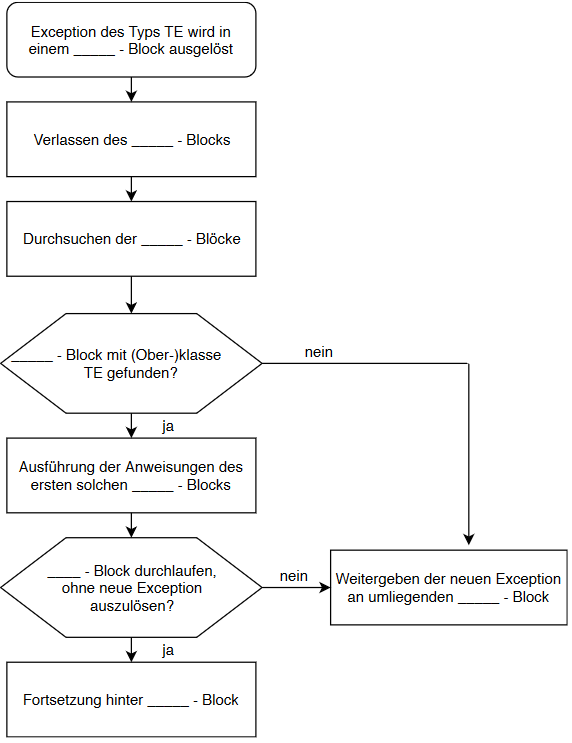
\includegraphics[width=\linewidth]{graphics/V4_Task.png}
    \end{minipage}

    \clearpagesolution

    \begin{solution}
      \begin{figure}[h]
        \centering
        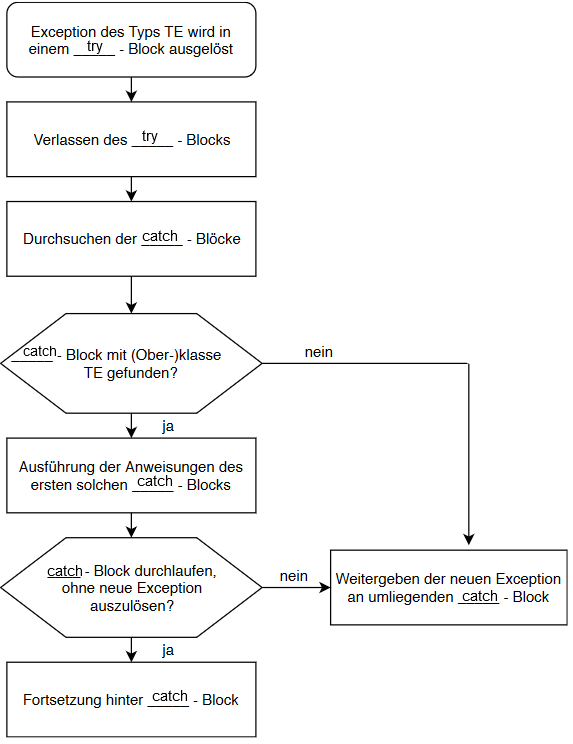
\includegraphics[width=.7\textwidth]{graphics/V4_Solution}
      \end{figure}
    \end{solution}
  \end{task}

  \clearpagesolution

  \begin{task}[credit=\stars{1}{3}]{assert-Anweisungen}
    In der Vorlesung haben Sie die assert-Anweisungen kennengelernt.
    \begin{enumerate}
      \item Beschreiben Sie in eigenen Worten, was ein Assertion-Error ist.
      \item Schreiben Sie den nachfolgenden Codeschnipsel kompakter mittels assert-Anweisungen!

      \lstinputlisting[style=Java]{codes/V5_Task.java}

      \item  Sie wissen, dass \inlinejava{assert}-Anweisungen beim Kompilieren an- oder
      abgeschaltet werden können mit entsprechenden Setzungen für den Compiler. Welche Vorteile
      ergeben sich hieraus? Warum sollten wir sie ausschalten und nicht einfach auch im realen
      Einsatz des Programms immer eingeschaltet mitlaufen lassen?
    \end{enumerate}

    \begin{solution}
      \begin{enumerate}
        \item Ein Assertion-Error ist ein Fehler, der so gewichtig ist, dass er mit
        Fehlerbehandlung nicht mehr zu retten ist. Deshalb soll das Programm dann sofort
        abgebrochen werden. Ein solcher Fehler wird mit Hilfe einer
        \inlinejava{assert}-Anweisung oder mit Hilfe eines \inlinejava{AssertionError} geworfen.
        \item\hfill
        \lstinputlisting[style=Java]{codes/V5_Solution.java}
        \item Beim Testen des Programms sind \inlinejava{assert}-Anweisungen sehr hilfreich, um
        mögliche Fehlerquellen schnell beheben zu können. Man sollte sie jedoch im realen Einsatz
        des Programms ausschalten, damit sich die Laufzeit des Programms nicht unnötig verzögert.
      \end{enumerate}
    \end{solution}

    \begin{note}[title=Information:]
      assert-Anweisungen sind standardmäßig nicht angeschaltet. Um diese verwenden zu können muss
      der Flag \inlinejava{-eq} für die JVM\footnote{Java Virtual Machine} hinzugefügt werden.
    \end{note}
  \end{task}

  \clearpage

  \begin{task}[credit=\stars{2}{3}]{Erster Test mittels BeforeEach}
    In dieser Aufgabe wollen wir einen Blick auf die \inlinejava{BeforeEach}-Annotation von JUnit
    5 werfen. Methoden mit dieser Annotation werden \textbf{vor Beginn jedes einzelnen Tests}
    ausgeführt!

    \br

    Gegeben sei eine Bibliothek für Geometrie-Funktionen. Dabei betrachten wir nur die Funktion
    \inlinejava{triangleArea}, die den Flächeninhalt eines Dreiecks berechnet und dazu die Längen
    der einzelnen Seiten  (\inlinejava{a}, \inlinejava{b} und \inlinejava{c}) als
    \inlinejava{int}-Werte übergeben bekommt.

    \begin{subtask*}{Setup vor jedem Test}
      Gegeben sei folgende Klasse \code{GeoLib}:

      \lstinputlisting[style=Java]{codes/V6_1_Task.java}

      Um die Funktionen der Bibliothek verwenden zu können, muss zunächst ein Objekt vom Typ
      \inlinejava{GeoLib} erzeugt werden. Hierzu können Sie den parameterlosen
      Standard-Konstruktor der Klasse \inlinejava{GeoLib} verwenden. Schreiben Sie eine
      entsprechend mit JUnit-Annotationen versehene Methode namens \inlinejava{setup}, die in
      einer Testklasse steht und die für jeden Testfall eine neue Instanz von \inlinejava{GeoLib}
      in dem bereits deklarierten Attribut \inlinejava{geoLib} speichert.

      \begin{solution}
        \lstinputlisting[style=Java]{codes/V6_1_Solution.java}
      \end{solution}
    \end{subtask*}

    \clearpagesolution

    \begin{subtask*}{Testfall}
      Schreiben Sie mindestens drei JUnit-Tests, die überprüfen, ob die Methode
      \code{triangleArea} für verschiedene Dreiecke korrekt arbeitet. Mindestens ein Testdreieck
      sollte dabei auch entartet sein.

      \begin{solution}
        \lstinputlisting[style=Java]{codes/V6_2_Solution.java}
      \end{solution}
    \end{subtask*}
  \end{task}

  \clearpage

  \begin{task}[credit=\stars{2}{3}]{Fehlertypen}
    In der Vorlesung haben Sie kennengelernt, dass man Fehler in Programmen in zwei Kategorien
    einteilen kann. Es wurde unterschieden zwischen Kompilierzeitfehlern und Laufzeitfehlern.

    \begin{enumerate}
      [label=(\arabic*)]
      \item Beheben Sie im folgenden Codeausschnitt alle Kompilierzeitfehler:
      \lstinputlisting[style=Java]{codes/V7_01_Task.java}
      \item Was passiert generell beim Aufruf der Methode \inlinejava{reverseArray}? Warum kann
      der Code auch ohne vorhandene Kompilierzeitfehler nicht fehlerfrei ausgeführt werden? Was
      müsste man beheben um den Code ausführbar zu machen?
      \item Das Programm läuft zwar jetzt fehlerfrei, das Ergebnis entspricht aber noch nicht dem
      gewünschten Ergebnis (Array soll umgedreht werden). Beheben Sie alle fehlerhaften Stellen
      im Code, um das gewünschte Ergebnis zu erreichen.
    \end{enumerate}

    \clearpagesolution

    \begin{solution}
      \begin{enumerate}
        [label=(\arabic*)]
        \item
        \begin{itemize}
          \item Zeile 1: \inlinejava{throws} statt \inlinejava{throws}
          \item Zeile 2: \inlinejava{source.length} statt \inlinejava{source.length()}
          \item Zeile 17: \inlinejava{Exception e}: \inlinejava{e} fehlt
        \end{itemize}

        \lstinputlisting[style=Java]{codes/V7_01_Solution.java}

        \clearpage

        \item
        \begin{itemize}
          \item Beschreibung:
          \newline
          Die Methode reverseArray hat die Funktionalität ein Array in umgekehrter Reihenfolge
          auszugeben. Dabei werden eine Variable, welche die Länge des Arrays zwischen speichert
          und zwei Laufzähler eingerichtet und das zurückzugebende Array wird deklariert. Im
          \inlinejava{try}-Block wird das zurückzugebende Array initialisiert. Die
          \inlinejava{while}-Schleife ist für das Invertieren zuständig. Wird eine
          \inlinejava{IndexOutOfBoundsException} oder jegliche andere Exception geworfen, so wird
          diese gefangen und eine Nachricht wird auf der Konsole ausgegeben.
          \item Fehler:
          \newline
          Der Code wird ohne Kompilierfehler nicht durchgehen. Die Gründe dafür sind:
          \begin{enumerate}
            \item Zeile 5: \inlinejava{j} soll auf das letzte Element des Arrays zeigen, aber
            dieses befindet sich am Index \inlinejava{length - 1}
            \item Zeile 12 + 13: Die Zählvariaben wurden falsch herum gesetzt und somit würde eine
            \inlinejava{IndexOutOf-BoundsException} geworfen werden, da hier \inlinejava{j}
            vergrößert und \inlinejava{i} verkleinert wird.
          \end{enumerate}
        \end{itemize}
        \lstinputlisting[style=Java]{codes/V7_02_Solution.java}

        \clearpage

        \item Das Problem ist, dass in der Zeile 21 und 22 das Ergebnis überschrieben wird,
        welches wir vorher berechnet haben. Um das Problem zu beheben wurden folgende Änderungen
        durchgeführt:
        \begin{itemize}
          \item Zeile 3: \inlinejava{inverted} wurde mit dem Wert \inlinejava{null}
          initialisiert, da die Methode in jedem Fall einen Wert zurückgeben muss.
          \item Zeile 23 und 24 wurden entfernt.
        \end{itemize}
        \lstinputlisting[style=Java]{codes/V7_03_Solution.java}
      \end{enumerate}
    \end{solution}
  \end{task}

  \clearpage

  \begin{task}[credit=\stars{2}{3}]{Testen mit JUnit - Qualitätskontrolle}
    Wir wollen ein neues System zur Qualitätskontrolle in einer Produktionskette testen. Hierzu
    gibt es eine Klasse
    \inlinejava{ProductLineManagement}, die Güter (Typ \inlinejava{Product}) herstellt. Ihre
    Tests sollen nun prüfen, ob dies schnell genug und hinreichend gut erfolgt. Die Maschinen
    garantieren dabei immer eine Mindestqualität von \(89\) (\(= 89\%\) der optimalen Qualität).

    \br

    Die Qualität wird gemessen auf einer Skala von \(0\) (defekt) bis \(100\) (perfekt).

    \br

    Die Testklasse deklariert ein Attribut \inlinejava{static ProductLineManagement plm}, auf das
    Sie zugreifen können.

    \begin{subtask*}{Setup-Methode}
      Vor jedem Test muss die (sehr komplexe) Produktionskette initialisiert werden. Dies erfolgt
      durch den Aufruf des Konstruktors der Klasse \inlinejava{ProductLineManagement} mit dem
      Namen der Firma als \inlinejava{String}. Den Firmennamen dürfen Sie beliebig wählen. Geben
      Sie eine mit JUnit-Annotationen versehene öffentlich sichtbare Methode an, die diese
      Initialisierung vor jedem Test durchführt.

      \begin{solution}
        \lstinputlisting[style=Java]{codes/V8_1_Solution.java}
      \end{solution}
    \end{subtask*}

    \begin{subtask*}{Normalfall}
      Schreiben Sie einen Test für eine normale Produktion. Hierbei soll ein einziger Artikel
      \inlinejava{normalProduct} durch die Methode \inlinejava{Product} \inlinejava{produce
        (String)} der Klasse \inlinejava{ProductLineManagement} (siehe oben) produziert werden.
      Stellen Sie sicher, dass der gelieferte Artikel nicht \inlinejava{null} ist und eine
      Mindestqualität - abfragbar via \inlinejava{getQuality()} - von \(89\) besitzt. Als Titel
      des Artikels können Sie einen beliebigen \inlinejava{String} angeben.

      \begin{solution}
        \lstinputlisting[style=Java]{codes/V8_2_Solution.java}
      \end{solution}
    \end{subtask*}

    \clearpagesolution

    \begin{subtask*}{Behandlung von Exceptions}
      Schreiben Sie nun einen weiteren Test, der auch wie im vorherigen Aufgabenteil ein neues
      Produkt erstellt. Nur diesmal reichen Sie dieses Produkt mittels
      \inlinejava{boolean submit(Product, int)} aus der Klasse
      \inlinejava{ProductLineManagement} für die Qualitätskontrolle ein. Wurde die gewünschte
      Qualität erreicht, liefert die Methode \inlinejava{true},  andernfalls wirft die Methode eine
      \inlinejava{InsufficientQualityException}.

      \br

      Testen Sie das Verhalten und das Auftreten der Exception mit einem Produkt, indem Sie
      dieses einmal auf die (garantierte) Mindestqualität von \(89\) und einmal auf die
      unerreichbare Qualität von \(101\) testen.

      \begin{solution}
        \lstinputlisting[style=Java]{codes/V8_3_Solution.java}
      \end{solution}
    \end{subtask*}
  \end{task}

  \clearpage

  \begin{task}[credit=\stars{2}{3}]{Testen: Racket und Java}
    Sie haben nun sowohl das Testen in Java mittels JUnit, als auch das Testen in Racket mittels
    Checks kennengelernt. In dieser Aufgabe sollen Sie zuerst eine Problemstellung in beiden
    Sprachen lösen und anschließend Ihre Implementierungen testen.

    \br

    Gegeben ist eine Zahlenliste. In Racket ist diese als Liste von \inlinejava{numbers} gegeben,
    in Java als Array von Typ \inlinejava{int[]}. Außerdem sind zwei Parameter \inlinejava{lower}
    und \inlinejava{upper} gegeben. Ziel ist es, alle Werte aus der Zahlenliste zu sortieren,
    welche nicht zwischen diesen beiden Grenzwerten \inlinejava{lower} und \inlinejava{upper}
    liegen (jeweils exklusive).

    \br

    Ergänzen Sie die beiden untenstehenden Codeausschnitte und Verträge, um diese Problemstellung
    zu lösen.

    \lstinputlisting[style=Racket]{codes/V9_01_Task.rkt}
    \lstinputlisting[style=Java]{codes/V9_02_Task.java}

    Sollte der Parameter \inlinejava{lower} dabei größer als der Parameter \inlinejava{upper}
    sein, so soll in Java eine
    \\
    \inlinejava{LowerBiggerThanUpperException}
    \\
    geworfen werden. Ergänzen Sie dies in Ihrer Implementierung.

    \br

    In Racket haben Sie die Möglichkeit einen Fehler auszulösen. Dies geschieht über den Befehl
    (\inlineracket{error} \inlineracket{msg}), wobei \code{msg} ein \inlineracket{String} mit der
    gewünschten Fehlermeldung ist. Konventionsmäßig einigen wir uns darauf, dass wir bei
    \inlineracket{msg} zuerst den Funktionsnamen nennen, gefolgt von einem Doppelpunkt und einer
    Beschreibung des Fehlers. Lösen Sie äquivalent zur \inlinejava{LowerBiggerThanUpperException}
    auch in der Racketfunktion einen Fehler für diesen Fall aus.

    \br

    Testen Sie abschließend die beiden Implementierungen mit jeweils 3 Tests. Ein Test sollte
    dabei das korrekte Werfen der Fehlermeldung testen.

    \clearpagesolution

    \begin{solution}
      \lstinputlisting[style=Java, lastline=21]{codes/V9_01_Solution.java}

      \clearpage

      \lstinputlisting[style=Java, firstline=23, firstnumber=22]{codes/V9_01_Solution.java}

      \clearpage

      \lstinputlisting[style=Java]{codes/V9_02_Solution.java}

      \clearpage

      \lstinputlisting[style=Racket]{codes/V9_Solution.rkt}
    \end{solution}
  \end{task}

  \clearpage

  \begin{task}[credit=\stars{2}{3}]{Exceptionklassen}
    \begin{subtask}
      Schreiben Sie eine \inlinejava{public}-Klasse \inlinejava{MyException}, die von
      \inlinejava{Exception} erbt. Der Konstruktor dieser Klasse hat einen Parameter
      \inlinejava{str} vom Typ \inlinejava{String} und einen Parametern vom Typ \inlinejava{int}.
      Ein Objekt von \inlinejava{MyException} hat ein \inlinejava{private}-Attribut
      \inlinejava{message} vom Typ \inlinejava{String}. Der Konstruktor weist
      \inlinejava{message} die Konkatenation aus beiden Parametern zu. Die
      \inlinejava{public}-Methode \inlinejava{getMessage} von \inlinejava{Exception} soll so
      überschrieben werden, dass \inlinejava{message} zurückgeliefert wird.

      \begin{solution}
        \lstinputlisting[style=Java]{codes/V10_1_Solution.java}
      \end{solution}
    \end{subtask}

    \begin{subtask}
      Schreiben Sie eine \inlinejava{public}-Klasse \inlinejava{X} mit einer
      \inlinejava{public}-Klassenmethode \inlinejava{km}, die einen \inlinejava{int}-Parameter
      \inlinejava{n} hat, \inlinejava{int} zurückliefert und potentiell \inlinejava{MyException}
      wirft. Und zwar wirft \inlinejava{km} eine \inlinejava{MyException} mit
      \code{\textcolor{stringcolor}{"'n cannot be negative"'}} und \inlinejava{n} als
      Parameterwerten, wenn negativ ist. Andernfalls liefert \inlinejava{km} das Quadrat von
      \inlinejava{n} zurück.

      \begin{solution}
        \lstinputlisting[style=Java]{codes/V10_2_Solution.java}
      \end{solution}
    \end{subtask}

    \begin{subtask}
      Schreiben Sie eine \inlinejava{public}-Klasse \inlinejava{Y} mit einer
      \inlinejava{public}-Objektmethode \inlinejava{m}, die einen \inlinejava{int}-Parameter
      \inlinejava{n} hat und \inlinejava{int} zurückliefert.
      Diese Methode ruft \code{km} von \inlinejava{X} mit \inlinejava{n} auf, ohne ein Objekt von
      \inlinejava{X} dafür einzurichten, und liefert das Ergebnis von \inlinejava{km} zurück.
      Sollte \code{km} eine \inlinejava{Exception} werfen, dann soll die Botschaft der
      \inlinejava{Exception} auf dem Bildschirm ausgegeben werden.

      \begin{solution}
        \lstinputlisting[style=Java]{codes/V10_3_Solution.java}
      \end{solution}
    \end{subtask}
  \end{task}

  \begin{task}[credit=\stars{3}{3}]{Welcher Belag darf es sein?}
    Schreiben Sie eine Klasse \inlinejava{NoBreadException} welche von \inlinejava{Exception}
    erbt, im Konstruktor einen Parameter \inlinejava{String} \inlinejava{topping} erhält und
    damit den Konstruktor der Basisklasse mit der Konkatenation
    \code{\textcolor{stringcolor}{"'There is no bread, only"'} +} \inlinejava{topping} aufruft.

    \br

    Schreiben Sie dann ein Functional Interface namens \inlinejava{Lunch}. Dieses enthält die
    funktionale Methode \inlinejava{String}
    \\
    \inlinejava{getTopping(String s)}, welche eine \inlinejava{NoBreadException} wirft.

    \br

    Initialisieren Sie nun das Functional Interface \inlinejava{Lunch} durch einen
    Lambda-Ausdruck. Geprüft werden soll, ob der \inlinejava{String} ein korrektes Sandwich ist.
    Dabei besteht ein korrektes Sandwich aus zweimal dem Substring
    \code{\textcolor{stringcolor}{"'bread}} und einem Topping dazwischen. Korrekte Sandwiches
    sind also beispielsweise \code{\textcolor{stringcolor}{"'breadtunabread"'}} oder
    \code{\textcolor{stringcolor}{"'breadabcdefgbread"'}}. Vordem ersten
    \code{\textcolor{stringcolor}{"'bread"'}} und nach dem zweiten
    \code{\textcolor{stringcolor}{"'bread"'}} darf kein Substring mehr stehen. Zurückgegeben
    werden soll immer das Topping, also der Substring zwischen den beiden
    \code{\textcolor{stringcolor}{"'bread"'}}'s. Das Topping muss dabei nicht \enquote{sinnvoll}
    sein, sondern irgendein beliebiger \inlinejava{String}. Ist kein Brot vorhanden, so soll eine
    \inlinejava{NoBreadException} mit dem alleinigen Topping geworfen werden.

    \br

    Sie dürfen davon ausgehen, dass niemals nur eine Brotscheibe verwendet wird, sondern entweder
    zwei oder keine.

    \clearpagesolution

    \begin{solution}
      \lstinputlisting[style=Java]{codes/V11_01_Solution.java}
      \lstinputlisting[style=Java]{codes/V11_02_Solution.java}
    \end{solution}
  \end{task}

  \clearpage

  \begin{task}[credit=\stars{3}{3}]{Arrays, Exceptions und Vererbung}
    \begin{subtask*}{Klasse X}
      \label{task:12.1}
      Gegeben sei die folgende Klasse:

      \lstinputlisting[style=Java]{codes/V12_1_Task.java}

      Wir benutzen das Array, auf das \inlinejava{a} verweist, um \inlinejava{int}-Werte zu
      speichern. Im Array, auf das \inlinejava{writable} verweist, wird festgehalten ob ein
      \inlinejava{int}-Wert in \inlinejava{a} überschrieben werden darf, oder nicht. Der
      \inlinejava{int}-Wert \inlinejava{a[i]} darf überschrieben werden, wenn
      \inlinejava{writable[i] == true}. Sie können davon ausgehen, dass beide Arrays der Klasse
      \inlinejava{X} immer die gleiche Länge besitzen, sodass die Indizes der beiden Arrays
      übereinstimmen.

      \br

      Implementieren Sie den Konstruktor der Klasse \inlinejava{X}, dieser bekommt einen
      \inlinejava{int}-Parameter übergeben und initialisiert die Arrays \inlinejava{a} und
      \code{writable} mit der gleichen Länge, dabei soll jeder Wert im Array
      \inlinejava{writable} mit \inlinejava{true} initialisiert werden. Die Länge beider Arrays
      entsprechen hier dem Wert des übergebenen Parameters. Erweitern Sie nun die Klasse um eine
      \inlinejava{public}-Methode \inlinejava{save}. Die Methode liefert nichts zurück, bekommt
      einen \inlinejava{int}-Parameter übergeben und speichert den übergebenen Parameter am
      kleinsten freien Index im Array \inlinejava{a} ab, an dem ein Wert nach aktueller
      Definition von \inlinejava{writable} überschrieben werden darf. Zusätzlich setzt sie den
      entsprechenden Wert im Array \inlinejava{writable} auf \inlinejava{false}. Darf kein Wert
      überschrieben werden, so soll die Methode eine \inlinejava{ArrayStoreException} mit der
      Nachricht \code{\textcolor{stringcolor}{"'no free space left"'}} werfen.

      \clearpagesolution

      \begin{solution}
        \lstinputlisting[style=Java]{codes/V12_1_Solution.java}
      \end{solution}
    \end{subtask*}

    \clearpagesolution

    \begin{subtask*}{Klasse Y}
      Schreiben Sie nun eine Klasse \inlinejava{Y}, die von der Klasse \inlinejava{X} aus Aufgabe
      \hyperref{task:12.1}{V12.1} erbt. Die Klasse soll die Methode \inlinejava{save} der
      Oberklasse überschreiben. Die Methode liefert nichts zurück, bekommt einen
      \inlinejava{int}-Parameter übergeben und soll mit diesem Parameter die Methode
      \inlinejava{save} der Oberklasse aufrufen. Wird dabei eine \inlinejava{ArrayStoreException}
      geworfen, so soll diese abgefangen werden. Ist dies der Fall, so sollen die beiden Arrays
      \inlinejava{a} und \inlinejava{writable} um ihre aktuelle Länge erweitert werden, um dann
      anschließend den übergebenen Parameter mittels der Methode \inlinejava{save} abspeichern
      zu können. Die bereits gespeicherten Werten in den beiden Arrays dürfen bei der Erweiterung
      nicht verloren gehen.

      \begin{solution}
        \lstinputlisting[style=Java]{codes/V12_2_Solution.java}
      \end{solution}
    \end{subtask*}
  \end{task}
\end{document}
